\chapter{Matemática Financeira}
\section{Juros Compostos}

\quest{Transpetro 2023 - CESGRANRIO}{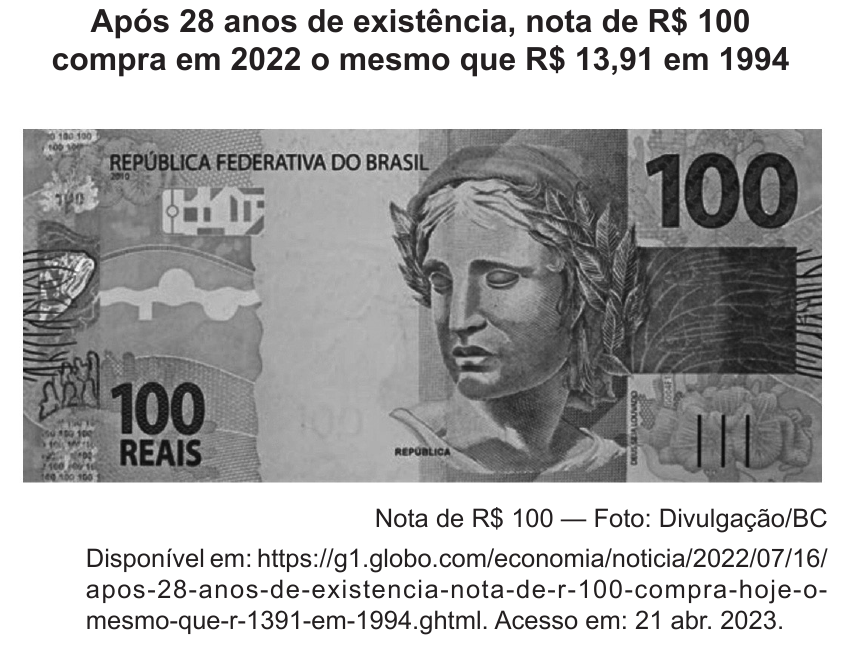
\includegraphics[scale=.5]{fig003.png}\\Suponha que, em 1994, um artigo custasse R\$ 13,91 e,
exatos 28 anos depois (336 meses), ele passasse a custar R\$ 100,00. Suponha, também, que, para esse período, a taxa mensal de aumento no preço desse artigo tenha sido igual a k\%, ou seja, a cada mês o preço do artigo sofreu um aumento de k\% em relação ao preço do mês anterior. O valor de k pode ser dado por}{
\item $100 \left(\dfrac{100}{13,91}\right)^{1/336}-100$
\item $100 \left(\dfrac{100}{13,91}\right)^{336}-100$
\item $\left(\dfrac{100}{13,91}\right)^{1/336}-1$
\item $\left(\dfrac{100}{13,91}\right)^{336}+0,01$
\item $100 \left(\dfrac{100}{13,91}\right)^{1/336}+0,01$
}{https://youtu.be/fDPDxc8zjzY}